%File: formatting-instruction.tex
\documentclass[letterpaper]{article}
\usepackage{aaai}
\usepackage{times}
\usepackage{helvet}
\usepackage{courier}
\usepackage{todonotes}
\usepackage{graphicx}
\usepackage{tabularx}
\usepackage{hyperref}
\frenchspacing
\pdfinfo{
/Title (Predicting Video Game Sales Using Metacritic Reviews: Critics vs Users)
/Subject (AAAI Publications)
/Author (anonymous)}
\setcounter{secnumdepth}{0}  
 \begin{document}
% The file aaai.sty is the style file for AAAI Press 
% proceedings, working notes, and technical reports.
%
\title{Predicting Video Game Sales Using Metacritic Reviews:\\Reviewers vs Users}
\author{anonymous\\
location\\
address 1\\
address 2\\
}
\maketitle

\begin{abstract}
\begin{quote}
Both professional critics and ordinary users provide reviews on a multitude of products, potentially providing valuable information about future product success. Previous work has typically analyzed user-provided reviews from large sales websites or specialized interest group forums. We instead address how critic and user review differ and how effective these review sources are for predicting sales. Using the relatively under-studied domain of videogames, we examine a corpus of review texts from the popular review site Metacritic and correlate features of these reviews to future videogame sales. Compared to critics, users skew towards providing higher scores, are the primary source of low scores, and show nearly equal expressions of sentiment in review text. A combination of critic scores, volume of critic reviews, and volume of user reviews in the 10 weeks prior to a game's release provides a moderately powerful model ($R^2 = 0.306$) for total game sales. Examining review texts, we find critics favor phrases describing the videogame market while users emphasize social aspects of playing games and the broader gamer culture. In sum, our work explores the differences between critic and user reviewers both in terms of their value as signals for product success and as representatives of different interest groups within the broad videogame product ecology.
\end{quote}
\end{abstract}


\section{Introduction}
Product reviews are often used by consumers as a purchase criteria. Particularly in the entertainment industry the opinions of an elite set of critics and journalists are often held as particularly important indicators of product quality. Professional film critics such as Roger Ebert are regarded as important guides to navigating the mass of films being released to recognize both hidden gems and over-hyped flops. Yet despite this widespread regard there is relatively little understanding of how indicative these critics' opinions are for market success of products. How effective are critic reviews for predicting future product sales? How do critic opinions compare to the opinions of regular consumers?

We address this question by comparing professional critics and amateur review website users in the task of predicting videogame sales. Are features of professional or amateur reviews more predictive of videogame sales? How does the power of grassroots word-of-mouth compare to the professional critical analysis? Do critics and users differ in their expressions of sentiment and does this effect their predictive power? How do professionals and amateurs describe products when reviewing? While previous research has often investigated the question of predicting sales from reviews, these efforts have focused on books \cite{gruhl2005predictive} or films \cite{dellarocas2007exploring} \cite{yu2012mining} \cite{duan2008online} \cite{liu2001word}, with little attention to the domain of videogames.
Further, few of these analyses have explicitly compared professional and amateur reviewers (see \cite{gilbert2010deja} for an examination of differences among amateur reviewers). Our analysis addresses a question at the heart of many contemporary debates: how does the crowd compare to domain specialists and where and when are each effective for predicting future outcomes?

For our analysis we gathered a corpus of 197,383 total reviews (138,843 from critics and 58,540 from users) from the review aggregation site Metacritic and sales data on 7467 games from the videogame sales tracking site VGChartz. Our data covers all information from these sites through December 7 2012. Metacritic collects reviews from print and online videogame review publications and produces an aggregate ``metascore'' reflecting a proprietary weighted combination of professional reviewer scores. Users are able to provide their own reviews for the same games. Anecdotally, many have claimed metascores can predict videogame success, at least when games cross a threshold of high enough score. First, we present an overview of our corpora that characterizes the distribution of professional and amateur review scores and sentiment expressions along with game sales. We use linear regression models to assess the predictive power of professional and amateur review scores for game total sales to date and sales over the first 10 weeks from being released. Our analysis includes using all review information and only a subset of reviews given prior to release of a game. Finally, we train classification models on review texts to find key words differentiating professional and amateur reviews showing different language and interests of the two groups. We find:
\begin{enumerate}
\item users are skewed toward higher review scores than critics, but users provide the main source of low review scores
\item users and critics show very similar levels of subjectivity and review polarity
\item a combination of mean critic score, volume of critic reviews, and volume of user reviews accounts is effective for predicting game sales
\item critics and users systematically differ in their reviews, with experts focusing on market and sales factors and users focusing on social aspects of playing the game
\item metascores are less important predictors than the volume of critic or user scores in a model combining information from metascores, critic, and user scores
\end{enumerate}


\section{Related Work}
The increasing prevalence and ease of access to social media data has led to a rise in research predicting real-world economic, political, and other events using \cite{asur2010predicting}. Predicting books sales \cite{gruhl2005predictive}, film box office sales \cite{dellarocas2007exploring}\cite{yu2012mining}, and (to a lesser extent) videogame sales from online reviews or blog chatter have all attracted attention \cite{ehrenfeld2011predicting}\cite{marcoux2009hybrid}. In early work in this area, Gruhl et al. demonstrated blog chatter can predict spikes in book sales rank on Amazon \cite{gruhl2005predictive}. 
Predicting box office sales has found volume of mentions on blogs or Yahoo!'s movie prerelease discussion forums can predictive film box office sales \cite{liu2001word}\cite{duan2008online}. Results conflict, however, on whether review score averages are \cite{dellarocas2007exploring} or are not \cite{liu2001word}\cite{duan2008online} predictive of sales, beyond the power of pure volume of reviews.
Sentiment has also often proven useful in predicting sales. Yu et al. found sentiment expressed in blog posts can improve an autoregressive model through a carefully chosen lexicon of sentiment-laden words \cite{yu2012mining}. Specialized classifiers that differentiate product description text from opinion related text were shown to improve sales prediction by Ghose and Ipeirotis \cite{ghose2007designing}. 
We address the question of review subjectivity and its relation to sales prediction and reviewer expertise, finding no strong predictive powers in the domain of videogame sales.

Few of these early works explicitly examine whether and how different types of reviewers produce varying review scores. Dellarocas et al. note a weak correlation between user and critic film reviews and find that removing critic review information (average score only) is slightly less detrimental to their model's performance than removing user review information (average score, number of reviews, entropy of review gender distribution, entropy of reviewer age distribution) \cite{dellarocas2007exploring}. Early works on review texts have characterized user reviewers in terms of their motivations for reviewing \cite{gilbert2010deja} and characteristic language used for describing videogame products in particular \cite{zagal2011natural}. We complement this work through an assessment of the differences between critic (professional) and user (amateur) reviewers through examining review volume, score, and sentiment rating in a linear model that allows direct comparison of predictive power. Further, our analysis of review text and score distributions provides more in-depth insight into how professional and amateur reviews differ. Rather than characterize user reviewer traits in isolation we seek to understand how they compare against professional critics.

Our work broadens previous analyses of videogame sales that have been limited to smaller subsets of games or sources for review data. Ehrenfeld's thesis found volume of game mentions on an online game discussion forum (NeoGAF\footnote{http://www.neogaf.com/forum/}) are predictive of game weekly sales in a support vector regression model. Marcoux and Selouani employed an autoregressive neural network model to predict games sales from review scores, volume, and related features using data from a single videogame news website (IGN \footnote{http://www.ign.com/}) after first performing nonlinear transformation on the model data. Compared to these approaches we examine a much larger set of games,\footnote{Ehrenfeld does not report the number of games used in his analysis, but limits to data over the course of 42 weeks of releases, which is a subset of our total corpus spanning 425 weeks. Marcoux and Selouani examine 74 games, while we examine 3000 or 600, depending on the model.} compare professional and amateur reviews, and draw from a longer-term and larger set of reviews that aggregate over websites. In contrast to previous non-linear models our results are directly interpretable in terms of relative feature impact in predictive models.


\section{Methodology}

\subsection{Corpus Collection}
\subsubsection{Metacritic reviews}
We used the python Scrapy package\footnote{http://scrapy.org/} to scrape all user and critic reviews for videogames from the Metacritic website\footnote{http://www.metacritic.com/} up through December 7 2012. For every game we collected the following information: console (the hardware the game software was made for), title, publisher (company responsible for distributing the game), developer (studio responsible for making the game), release date, current metascore, current average user score, genre (according to Metacritic), and ESRB rating (age-appropriateness rating). Note that some titles may appear on multiple consoles. We treat these as separate games as they reach potentially different audiences and may vary in their implementation. From every game we also collected all user and critic reviews, including their text, review score, time of review, and a flag indicating whether the review came from a user or critic. Metacritic converts critic review scores from many formats (such as letter grade, 0-10 range, 0-100 range) into a 0-100 score. User reviews are limited to a 0-10 score range. For comparison we divide all critic scores by 10 to have all reviews on a [0-10] scale. Metacritic only provides summary excerpts from critic reviews and we limited ourselves to this text to make review length more comparable between users and critics. Our final corpus consists of 197,383 reviews: 138,843 from critics and 58,540 from users. Of these, 45,679 critic and 58,531 user reviews had review date time stamps; this subset of reviews were used in our prediction tasks.

\subsubsection{VGChartz sales data}
For sales data we scraped information from the VGChartz website\footnote{http://www.vgchartz.com/}. VGChartz tracks game weekly, annual, and lifetime sales data from a variety of outlets and is primarily targeted toward sales of games in the United States. Their data is most accurate for console games (rather than computer or mobile phone), so we limit ourselves to examining the following consoles using only US sales data: Sony's PlayStation 3 (PS3), PlayStation Portable (PSP) and Vita; Nintendo's Wii, DS, and 3DS; and Microsoft's Xbox360. These consoles are considered to make up the current generation of videogame hardware and are the primary game console distribution platforms. For weekly data VGChartz typically only records the first 10 weeks of game sales, and so our time series analysis is limited to these weeks. We collected total lifetime sales-to-date for 7467 games and weekly sales for the first ten weeks of game sales for 4902 games.

\subsection{Methods}
\subsubsection{Sales prediction regression}
Our analysis involved two components: (1) predicting game sales (both lifetime and over the first 10 weeks of sales) and (2) identifying words distinguishing critic and user reviewers. Sales predictions investigated: (1) predicting total lifetime sales-to-date using the full review database, (2) predicting total lifetime sales-to-date using only reviews in the 10 weeks prior to the release of a game, (3) predicting net first 10 week sales using the same pre-release review subset, and (4) predicting lifetime sales using the full review database augmented with metascore information (Table \ref{tab:regression_models} summarizes our models). Predictive accuracy was assessed through mean squared error computed with leave-one-out cross-validation through bootstrapped resampling with R's boot package\footnote{http://cran.r-project.org/web/packages/boot/}.
%To predict lifetime sales data we constructed a robust linear regression model for logged lifetime game sales based on median review scores using R's MASS package\footnote{http://cran.r-project.org/web/packages/MASS/}.

\todo[inline]{needs cleanup}
\begin{table}[tb]
\centering
\scriptsize
\begin{tabularx}{\linewidth}{|c|c|X|X|X|X|X|X|}
\hline\textbf{ predicted variaable} & \textbf{review set} & \textbf{number games} & $R^2$ & MSE & null deviance & control deviance & model deviance \\ 
%\hline lifetime sales-to-date & all user and critic reviews & 6809 & 0.405 & 0.600 & 6807.2 & 6129.5 & 4047.9\\ 
%\hline lifetime sales-to-date & user and critic reviews in 10 weeks prior to release & 600 & 0.360 & 0.669 & 562.43 & 500.49 & 359.73\\ 
%\hline net first 10 week sales & user and critic reviews in 10 weeks prior to release & 600 & 0.421 & 0.642 & 599.00 & 502.08 & 346.8\\ 
%\hline lifetime sales-to-date & all metascores, user, and critic reviews & 839 & 0.442 & 0.588 & 838.72 & 735.73 & 467.99\\ 
\hline lifetime sales-to-date & all & 6809 & 0.405 & 0.600 & 6807 & 6130 & 4048\\ 
\hline lifetime sales-to-date & pre-10 & 600 & 0.360 & 0.669 & 562 & 500 & 360\\ 
\hline net first 10 week sales & pre-10 & 600 & 0.421 & 0.642 & 599 & 502 & 347\\ 
\hline lifetime sales-to-date & meta & 839 & 0.442 & 0.588 & 839 & 736 & 468\\ 
\hline 
\end{tabularx}
\caption{Linear regression models. Review set indicates which subset of reviews were used: ``all'' indicates using the full review database, ``pre-10'' indicates only reviews from the 10 weeks prior to the launch of the game, and ``meta'' indicates the full review database and metascore information. Mean squared error (MSE) values are from leave-one-out cross-validation of models. Null deviance reports null model deviance; control deviance includes only control, game genre, and ESRB rating as predictors; model deviance uses full set of predictive variables including controls.}
\label{tab:regression_models}
\end{table}

After matching game reviews to sales data using game titles and consoles we had lifetime sales data for 2909 games, and weekly sales for 600 games. We used a conservative approach of only keeping exact game title matches without manipulating titles (e.g. using lowercase versions or removing punctuation). In our case it is better to have a slightly smaller dataset than misattribute review scores to different sales. We predicted both full lifetime sales-to-date and summed weekly game sales data over the first 10 weeks of available information. Sales values were logged to ensure normality. Reviews and sales data were aligned based on weeks since release. Reviews were binned into weekly periods based on time since the release of the game. For example, all reviews within 7 days of the game's stated release date (for that console) were binned into the first week. We employed a simple linear regression model for better model result interpretability. Our model incorporated features for mean and median review scores, number of reviews, mean and median review text polarity, and mean and median review text subjectivity. Review polarity and subjectivity were computed on the per-sentence level, aggregated (mean, median, or maximum) per review, and then aggregated (mean or median) across reviews per game. These multiple perspectives allowed us to consider expressions of average review sentiment, skew in review sentiment, or extreme review sentiment.

\subsubsection{Review sentiment extraction}
We employed python's pattern package\footnote{http://www.clips.ua.ac.be/pages/pattern} to analyze review text sentiment. For every review text we parse the text into sentences, compute per-word sentiment (both polarity and subjectivity) and compute the per-review mean, median, and maximum sentiment values. Subjectivity values measure to what extent a text conveys an opinion. Polarity values estimate that valence as positive or negative. Below we refer to these per-sentence aggregation values as the review ``mean'', ``median'' or ``maximum'' polarity or subjectivity.

\subsubsection{Reviewer text analysis}
%Our analysis of review text examined the predictive power of review text words to: (1) distinguish reviewers as critics or users; (2) predict review score; and (3) distinguish game consoles being described. 
Our analysis of review text examined the predictive power of review text words to distinguish reviewers as critics or users (labeled 0 and 1, respectively) using penalized binomial regression with a lasso penalty to favor the use of a small set of terms. 
We prepared our review texts using several standard methods performed in text analysis using the R programming language packages tm\footnote{http://cran.r-project.org/web/packages/tm/} and topicmodels\footnote{http://cran.r-project.org/web/packages/topicmodels/}. We removed whitespace, punctuation, numbers not part of words, and common English words (known as stopwords). All text was lowercased and stemmed to group together repeated use of similar words. We tokenized these documents into single words, requiring words be at least 3 letters long and appear in at least 10 documents. After constructing a full corpus of 86,376 terms we removed the most sparse terms to produce a set of 2,581 terms.

Binomial regression was performed using R's glmnet package\footnote{http://cran.r-project.org/web/packages/glmnet/} for generalized linear models. These models account for collinearity of terms (their frequent appearance together altering relative importance) and can control for sparsity (relative infrequency of terms). Controlling collinearity is important to prevent overweighting words that often appear together. Accounting for sparsity enables the model to exclude terms with little predictive power, yielding a smaller and more interpretable set of results. This was done using a lasso penalty that encourages the model to use the smallest set of terms possible


\section{Results}

\subsection{Corpus Overview}
Before describing results on our prediction tasks it is important to understand the characteristics of the review and sales corpuses we collected. Metacritic users are not necessarily representative of the opinions of all those interested in videogames and it is not apparent \textit{a priori} how they behave compared to the critics whose reviews are featured on the site.

\subsubsection{Review scores}
Users and critics show clear differences in review score attribution (Figure \ref{fig:revscore_console}). Critics tend to provide reviews distributed more tightly around a mean 7.2 and median 7.5 score, while users show more variation with a mean 7.4 and median 9.0 score. A Wilcoxon test found these differences to be significant (p $< 0.001$). Also note that users favor providing higher scores than critics, but are the only ones likely to provide low review scores.
Intuitively these results make sense. Critics are often under threat of blacklist for providing low review scores and have a reputation to preserve by not consistently giving high review scores. Game distributors are also unlikely to provide reviewers with free game copies for review if they anticipate low ratings, while critics are unlikely to review low profile and low quality titles. These factors combine to skew critics towards reviewing games generally favorably without providing overly positive reviews. Users, in contrast, are most likely to review when a game provided a great or terrible experience. As Metacritic is a major game review outlet reviewers are likely to provide high scores to games they enjoyed, while attacking games they found poor quality or a waste of money.

\begin{figure}[tb]
\centering
%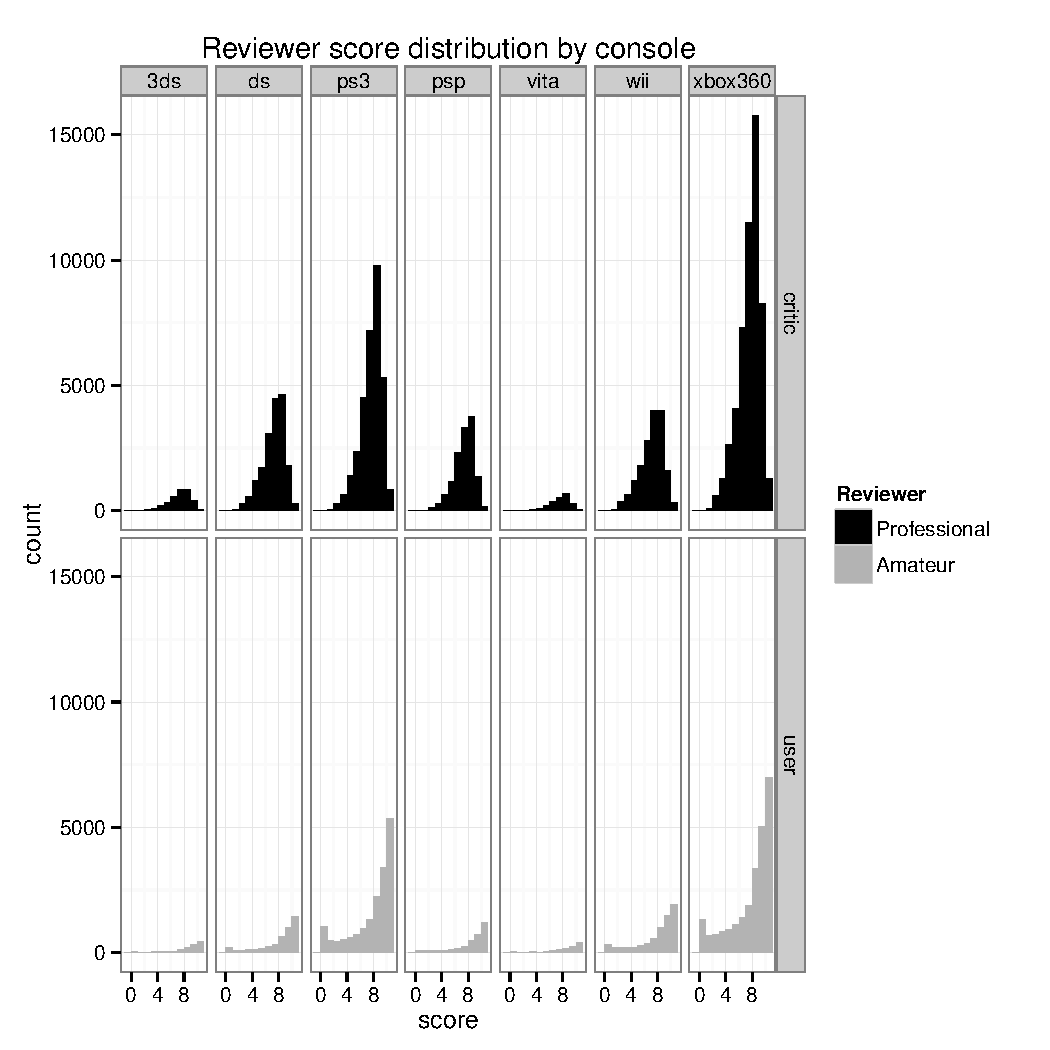
\includegraphics[width=\linewidth]{./console_reviews_score_hist}
%\caption{review score distribution by console}
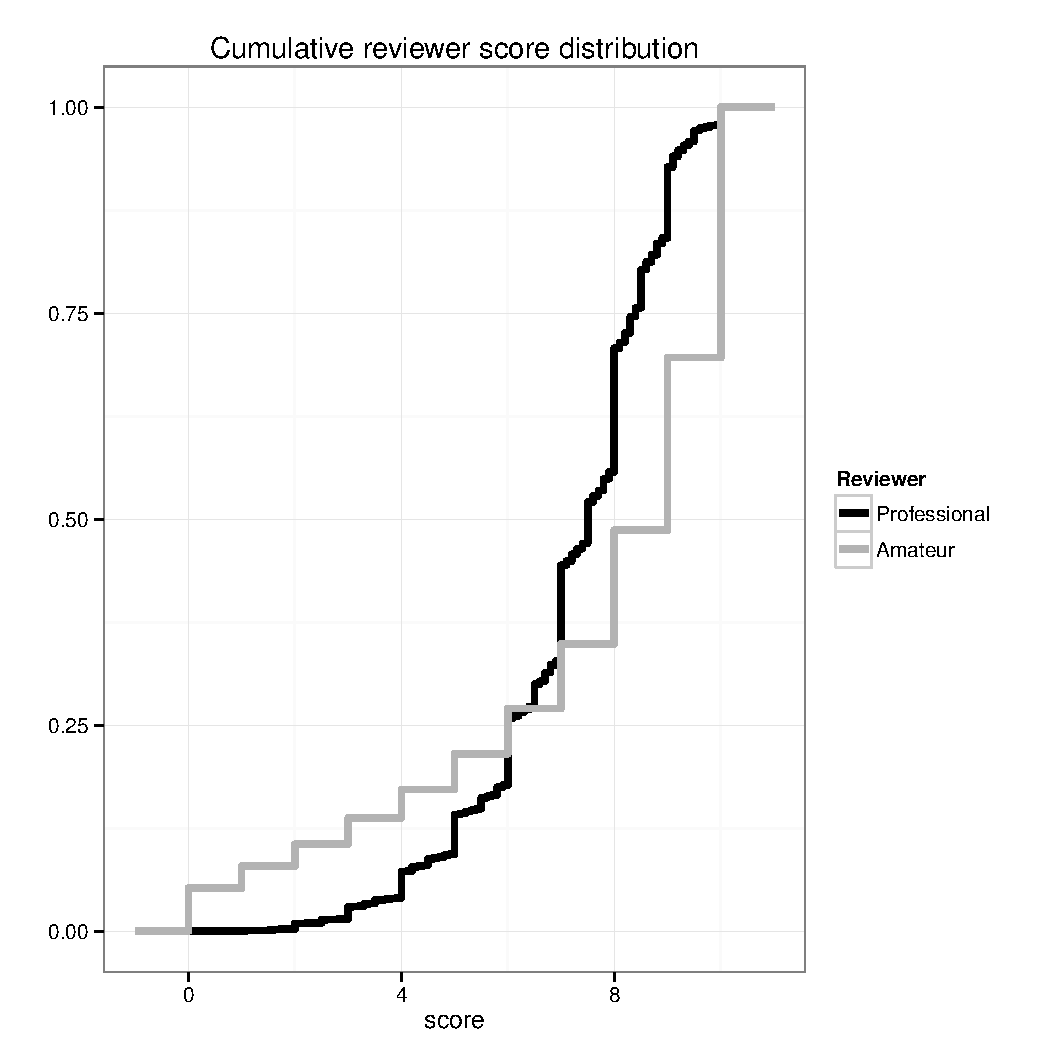
\includegraphics[width=\linewidth]{./console_reviews_score_ecdf}
\caption{Cumulative review score distribution by console}
\label{fig:revscore_console}
\end{figure}

\subsubsection{Review sentiment}
Reviewers and critics also show different levels of subjectivity and polarity in reviews (Figures \ref{fig:revpol_density} and \ref{fig:revsubj_density}). For our analysis we consider median polarity and subjectivity values over all review scores; all results reported were significant according to a Wilcoxon test at p $< 0.001$, although these differences may not appear in Table \ref{tab:review_pol_subj} when rounding to two decimal places. 
Both critics and user review distribution are slightly skewed by the presence of larger numbers of high polarity and subjectivity reviews (compare means and medians in Table \ref{tab:review_pol_subj}). Critics tend to give lower scores and show less skew in review scoring---7.2 mean and 7.5 median for critics, 7.4 and 9.0 for users. Critics thus tend to be more consistent in scoring and more conservative about providing overly positive reviews.
Users are more likely to employ at least one sentence that is strongly subjective and of more positive valence than critics. Both users and critic reviews are skewed towards moderately positive sentiments, although most cluster around neutral tones (Figure \ref{fig:revpol_density}). 

\begin{table}
\scriptsize
\begin{tabularx}{\linewidth}{|c|X|X|X|X|}
\hline  & \multicolumn{2}{|c|}{\textbf{critics}} & \multicolumn{2}{|c|}{\textbf{users}}  \\ 
\hline \textbf{review attribute} & \textbf{mean} & \textbf{median} & \textbf{mean} & \textbf{median} \\ 
\hline score & 7.2 & 7.5 & 7.4 & 9.0 \\ 
\hline mean polarity & 0.14 & 0.12 & 0.15 & 0.13 \\ 
\hline median polarity & 0.14 & 0.10 & 0.12 & 0.00 \\ 
\hline max polarity & 0.25 & 0.22 & 0.51 & 0.50 \\ 
\hline mean subjectivity & 0.50 & 0.50 & 0.48 & 0.48 \\ 
\hline median subjectivity & 0.50 & 0.50 & 0.47 & 0.50 \\ 
\hline max subjectivity & 0.65 & 0.69 & 0.86 & 1.00 \\ 
\hline 
\end{tabularx}
\caption{Comparison of critic and user review text sentiment.}
\label{tab:review_pol_subj}
\end{table} 

While differences in polarity and subjectivity were significant, their magnitude was small. Contrary to our expectations, critics are not particularly objective when compared to users, except in terms of the most polarizing sentences used in their reviews. One limitation of this interpretation, however, is that critic texts were limited to summaries and thus may not reflect the intended valence of the review, but a revised summary meant to convey factual information for the purposes of featuring on Metacritic. These results may also reflect limitations of our sentiment analysis itself and merit further investigation using full review texts from the original review sites.


\begin{figure*}[tb]
\centering
%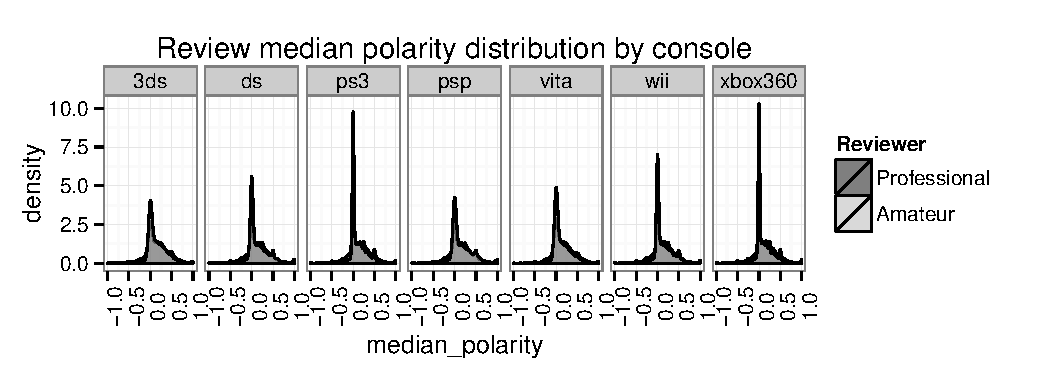
\includegraphics[width=\linewidth]{./console_reviews_polarity}
%\caption{review polarity density by console comparing reviewer type}
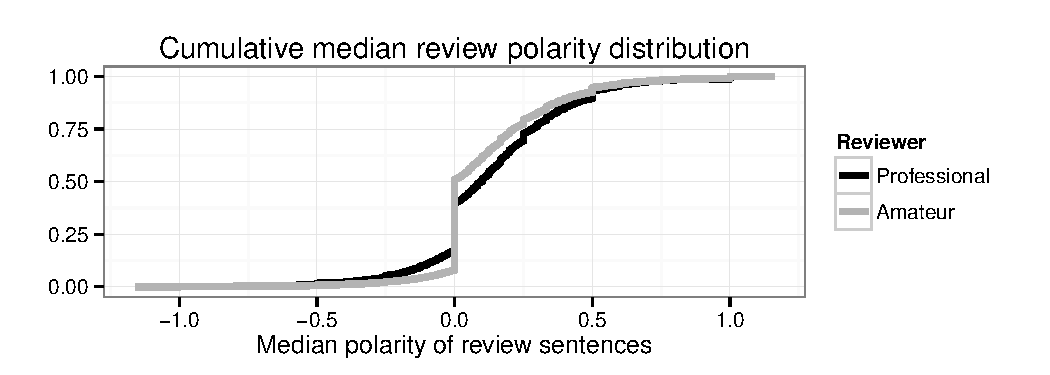
\includegraphics[width=\linewidth]{./console_reviews_polarity_ecdf}
\caption{Cumulative review polarity distribution by console comparing reviewer type}
\label{fig:revpol_density}
\end{figure*}


\begin{figure*}[tb]
\centering
%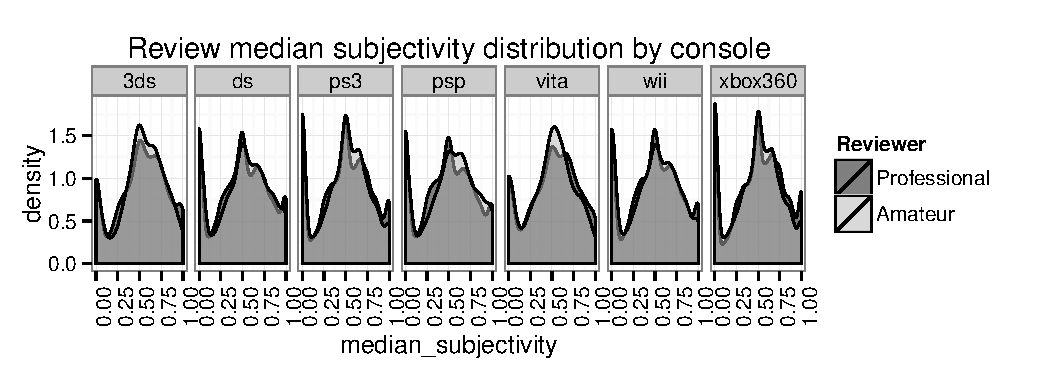
\includegraphics[width=\linewidth]{./console_reviews_subjectivity}
%\caption{review subjectivity density by console comparing reviewer type}
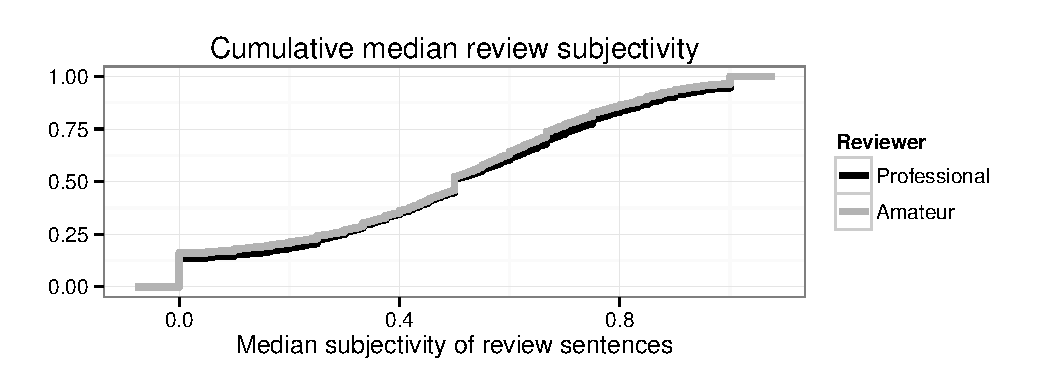
\includegraphics[width=\linewidth]{./console_reviews_subjectivity_ecdf}
\caption{Cumulative review subjectivity distribution by console comparing reviewer type}
\label{fig:revsubj_density}
\end{figure*}



\subsection{Sales Prediction}
We used linear models to predict mean lifetime sales for each game, controlling for game console, genre, and ESRB maturity rating. While linear models may have limited predictive power for nonlinear relationships they afford direct interpretation useful to analysts employing the results. We examined models for predicting game sales-to-date and net first ten week sales considering a set of factors: review author (critic or user), review scores, number of reviews, and review text features (length, polarity, subjectivity). We examined four models: predicting total sales from all reviews, predicting total sales from reviews in the 10 weeks prior to the game's release, and predicting net first 10 week sales from the same pre-release review subset. Table \ref{tab:regression_models} summarizes the models; Tables \ref{tab:sales_allmodel_lm} and \ref{tab:sales_metascore_lm} summarize the predictive variables, standardized $\beta$ coefficients, and model fitting results for each model.

\begin{figure}[tbp]
\centering
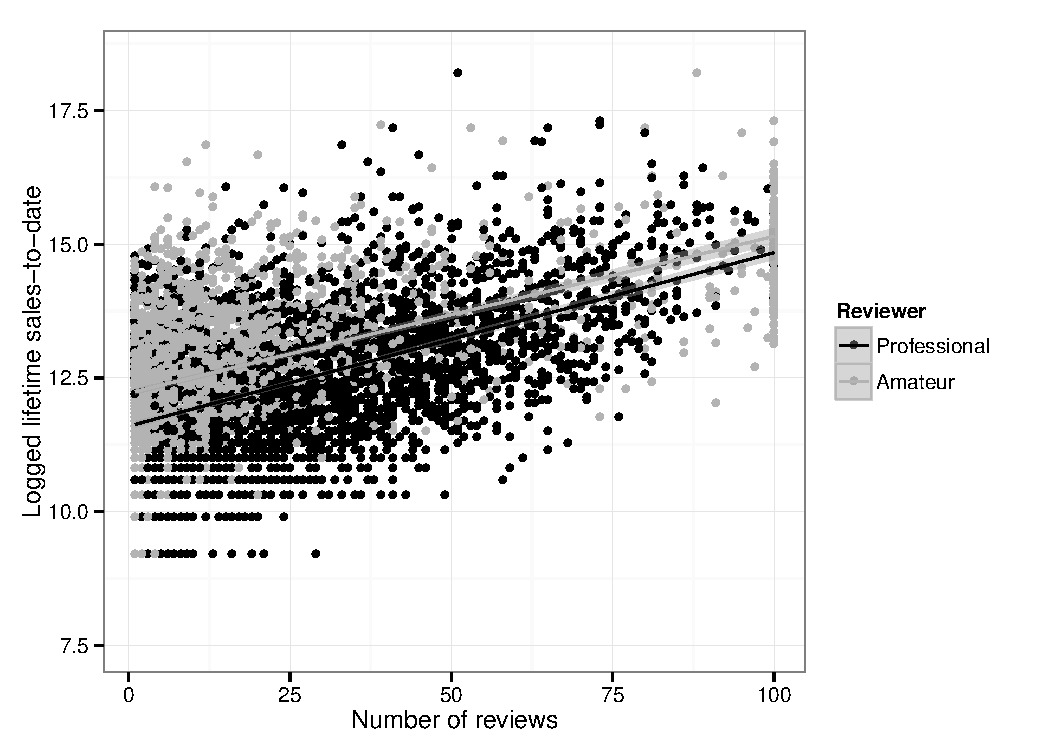
\includegraphics[width=\linewidth]{./sales_numscore_total}
\caption{Lifetime sales-to-date vs number of reviews by reviewer type}
\label{fig:lifesale_revnum}
\end{figure}

\begin{figure}[tbp]
\centering
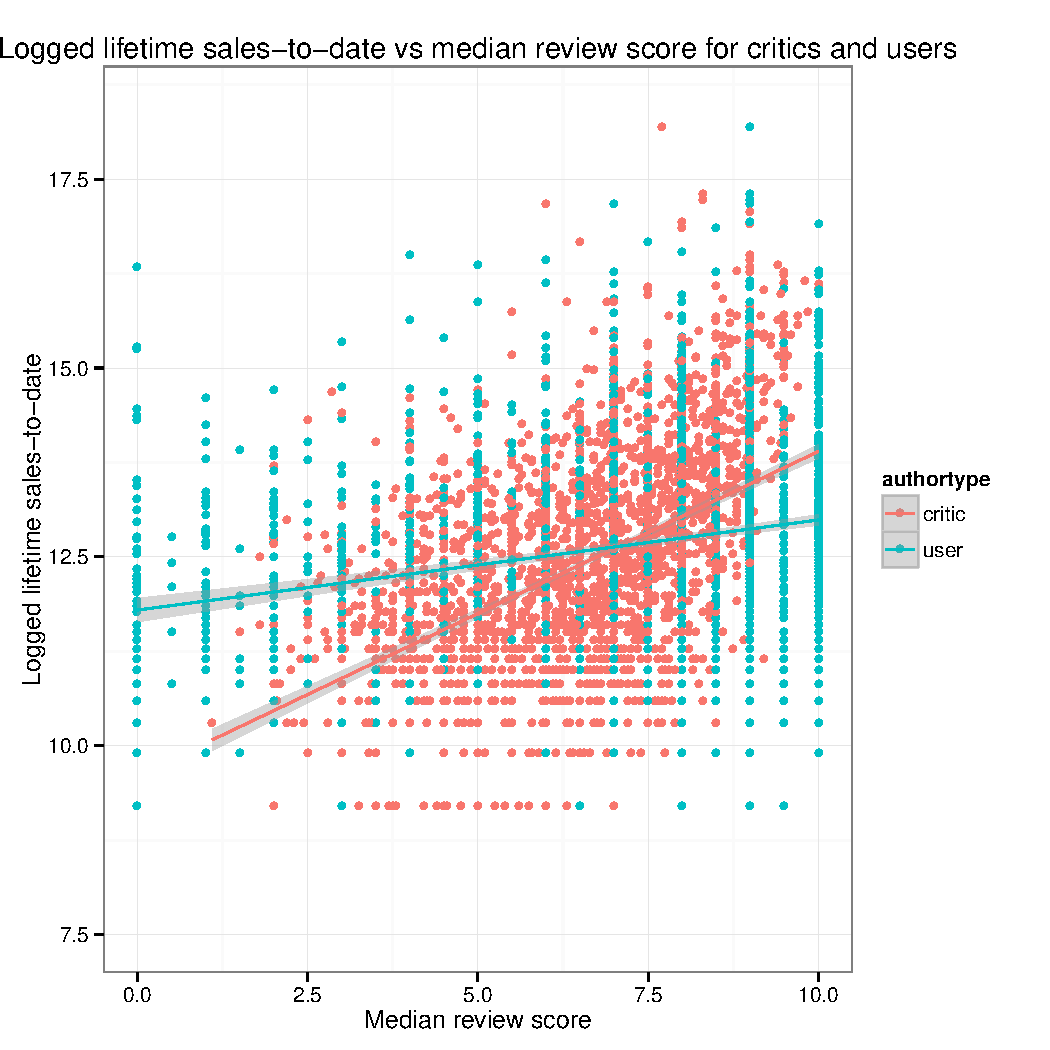
\includegraphics[width=\linewidth]{./sales_medianscore_total}
\caption{Lifetime sales-to-date vs median review score by reviewer type}
\label{fig:lifesale_revscore}
\end{figure}

Review scores and volume show clear relationships to the lifetime sales of a game (Figures \ref{fig:lifesale_revnum} and \ref{fig:lifesale_revscore}). Anecdotally many have claimed that a metascore over 90 (9 on our rescaled range) leads to a substantial boost to game sales. Our data supports this notion when looking only at aggregated critic scores, although the range of relevance is broader (Figure \ref{fig:lifesale_revscore_boxplot}).\footnote{We found similar trends when examining Metascores, although the dataset is limited to fewer games.} User scores do not show a clear relationship to sales: increasing median user review score does not appear to relate to any substantial gain in scores. By contrast, critic review scores show a clear increasing relationship, starting around scores above 60 but becoming most prominent for scores above 80. While the [95-100] category has only 25 critic reviews and thus is of dubious predictive value, the [85-90] and [90-95] categories consist of 371 and 56 reviews and thus are of greater predictive merit.

\begin{figure}[tbp]
\centering
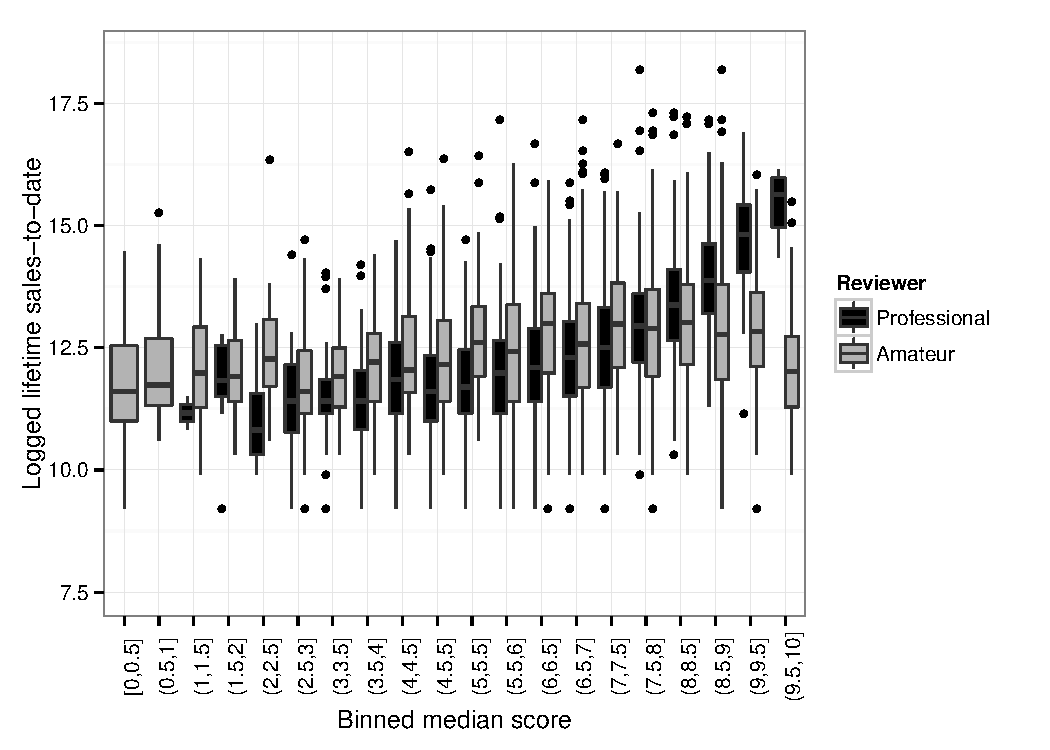
\includegraphics[width=\linewidth]{./sales_binnedscore_vs_total}
\caption{lifetime sales vs binned review scores}
\label{fig:lifesale_revscore_boxplot}
\end{figure}

\subsubsection{Total sales vs all reviews}
\todo[inline]{update numbers to match tables: tables are correct}
Our models show moderately strong predictive power ($R^2$ between $0.275$ and $0.390$, MSE between $0.668$ and $0.757$) for logged sales (Tables \ref{tab:sales_allmodel_lm} and \ref{tab:sales_metascore_lm}). All regressors were converted to standardized scores by subtracting their means and dividing by their standard deviations. Regression results report only significant ($p < 0.001$) standardized $\beta$ coefficients.

For each model we computed all possible linear models formed from subsets of review score and text features and scored them according to the Bayesian Information Criterion (BIC) using R's leaps package.\footnote{http://cran.r-project.org/web/packages/leaps/} Using the BIC allows our model selection process to penalize overly complex models to reduce the likelihood of overfitting. Relative importance of model parameters was measured using the lmg metric in R's relaimpo package.\footnote{http://cran.r-project.org/web/packages/relaimpo/} The lmg metric calculates the average $R^2$ contribution averaged over orderings among predictive variables---we use relative values among predictors to compare their importance.

\todo[inline]{update with controlled cross-validated numbers}
For total sales we examined a model treating critic and user reviews as separate sources of predictors, looking only at games with data from both groups and using all reviews in our dataset (6809 games). The BIC identified the following variables (relative importances summing to 100\% across regressors, including controls, are reported in parenthesis): mean critic review score (15.80\%), mean user review score (2.53\%), number of critic reviews (27.49\%), number of user reviews (37.43\%), mean user review length in characters (4.92\%), median of per-review maximum subjectivity from critic reviews (0.86\%), mean of the same from user reviews (0.36\%). Overall the model's adjusted $R^2$ value of $0.3904$ and MSE of $0.668$ suggests a strong correlation between these factors and lifetime sales.
%We compared this model against those ablating one or more of the predictive variables and found the differences significant according to an ANOVA ($p < 0.05$), confirming this model includes only statistically meaningful variables.

\begin{table}[tb]
\centering
\scriptsize
\begin{tabularx}{\linewidth}{|X|c|c|}
\hline  & \multicolumn{2}{|c|}{\textbf{total vs all reviews} ($R^2 = 0.390$)}\\ 
\hline \textbf{variable} & \textbf{$\beta$} & \textbf{relative importance}\\ 
\hline mean critic score & 3.084e-01 & 30.85\%\\ 
\hline mean user score & -6.273e-02 & 2.53\%\\ 
\hline number critic reviews & 1.729e-01 & 27.49\%\\ 
\hline number user reviews & 3.165e-01 & 37.43\%\\ 
\hline mean user review length & -4.592e-02 & 0.49\%\\ 
\hline median(max review subjectivity) critics & -6.431e-02 & 0.86\%\\ 
\hline median(max review subjectivity) users & -4.462e-02 & 0.36\%\\ 
\hline 
\end{tabularx}
\caption{Regression models for lifetime sales-to-date using all available reviews. $\beta$ are standardized regression coefficients when predicting log-scaled and standardized lifetime sales. All values are significant at $p < 0.001$. \textbf{MAY CUT THIS ANALYSIS ALTOGETHER}}
\label{tab:sales_totsale_lm}
\end{table}

\todo[inline]{of control variables, esrb is always significant, as is platform, sometimes genre}
%\begin{table}[tb]
%\centering
%\scriptsize
%\begin{tabularx}{\linewidth}{|X|c|c|}
%\hline  & \multicolumn{2}{|X|}{\textbf{total vs all reviews} ($R^2 = 0.4053$, $MSE = 0.59995$)}\\ 
%\hline \textbf{variable} & \textbf{$\beta$} & \textbf{relative importance}\\ 
%\hline median score & 0.30145 & 15.80\%\\ 
%\hline number of reviews & 0.53365 & 53.32\%\\ 
%\hline reviewer type (as user) & 0.37623 & 4.79\%\\ 
%\hline reviewer type (as user) X median score & -0.21179 & 2.60\%\\  
%\hline reviewer type (as user) X mean(mean review polarity) & 0.03635 & 2.31\%\\ 
%\hline reviewer type (as critic) X mean(mean review subjectivity) & -0.02785 & 0.17\%\\ 
%\hline 
%\end{tabularx}
%\caption{Regression model for lifetime sales-to-date comparing metascores, users, and critics. $\beta$ are standardized regression coefficients when predicting log-scaled and standardized lifetime sales. All values are significant at $p < 0.001$ except median(median review subjectivity) which is marginally significant at $p < 0.1$.}
%\label{tab:sales_allreview_lm}
%\end{table}

As expected from the previous distributions, review subjectivity is a weak factor for predicting total sales. Sheer volume of user and critic reviews account for the largest part of our model's power. Intuitively this makes sense: volume of critic and user reviews both reflect relative attention to a game and also likely reflect the relative publishing and marketing resources behind the game's developer. More user reviews reflect games more people have played (and thus likely already purchased). Further, games that drive users to respond on online forums reflect greater social popularity. Greater volume of critical reception similarly reflects publisher budget and expectations. Review copies are typically distributed to critics when publishers expect games to be reviewed well, bolstering their review numbers. Further, only more well-financed and established publishers are able to push their games to be reviewed by venues that metacritic would index and report from.

While critic scores and number of reviews have roughly equal relative importance, user scores are relatively unimportant. Given the distributions seen above this makes sense: games that have many user reviews are rare, but enjoy strong sales on average. For a game to have many user reviews requires many users to have played the game and been motivated to review the game. From the previous distributions of review scores we would expect these reviewers to (mostly) give positive scores, thus the fact that they are writing a score at all is indicative of what that score will be. Playing the game typically means a user has purchased the game, thus further entangling with sales. While direct causality cannot be read off from these results it is clear that the amount of attention users or critics devote to a game is indicative of its level of sales success. Future work should explore more sophisticated features for predicting sales such as reviews in the weeks prior to launch, number of reviews in the first weeks of sales (not just overall), or volume of previews. Twitter, Facebook, and Youtube and other media consumption information (not necessarily reviews) may be important gauges of broad consumer interest that complements the more devoted group of Metacritic user reviewers.

\subsubsection{Total and net 10 week sales vs pre-release reviews}
For the purpose of predicting future sales we examined a model that aggregated reviews only in the 10 weeks prior to the release of a game and used this data set to predict lifetime sales-to-date. Due to sparsity of games (600 total) that possessed both critic and user reviews in this period we altered the form of the model to use the same predictive variables as above but with a dummy variable indicating review type and adding terms to assess interaction effects between this variable and the other regressors. With an adjusted $R^2$ of $0.275$ and leave-one-out cross-validated mean squared error of $0.718$ the model is less powerful than before. Relative variable importance mirrors the prior results: number of reviews (42.78\%), median review score (31.59\%), reviewer type flag (20.63\%), interaction effect between reviewer type and number of reviews (1.18\%), interaction effect between reviewer type and median score (3.83\%); interaction effects between mean of per-review mean polarity and mean of per-review mean subjectivity were both unimport (0.00\%). Directionally these results have the same message: volume of reviews is most important, followed by receiving favorable review scores, with all other factors playing a relatively minor role. Knowing users are providing review scores lowers the estimated effect on sales while knowing more users are writing reviews raises the estimate effect on sales. We created an analogous model predicting net sales over the first 10 weeks, achieving an adjusted $R^2$ of $0.306$ and MSE of $0.718$. Results were qualitatively the same as the total sale model, refer to Table \ref{tab:sales_allmodel_lm} for details. This is not surprising as most game sales occur during the initial launch and marketing period, with relatively few games having more long-term strong sales or shifts in sales.

%\begin{table*}[tb]
%\centering
%\scriptsize
%\begin{tabular}{|l|c|c|c|c|}
%\hline & \multicolumn{2}{|c|}{\textbf{10 week vs pre-10}} & \multicolumn{2}{|c|}{\textbf{total vs pre-10}}\\ 
%\hline \textbf{variable} & \textbf{$\beta$} & relative importance & \textbf{$\beta$} & relative importance\\ 
%\hline median review score & 0.64691 & 18.63\% & 0.553424 & 19.88\%\\ 
%\hline number of reviews & 0.23578 & 21.06\% & 0.235556 & 20.88\%\\ 
%\hline reviewer type (as user) & 0.43711 & 2.60\% & 0.606100 & 10.76\%\\ 
%\hline reviewer type (as user) X median score  & -0.61708 & 12.93\% & -0.505708 & 11.01\%\\ 
%\hline reviewer type (as user) X number of reviews & 0.51815 & 1.98\% & 0.431584 & 1.76\%\\ 
%\hline reviewer type (as user) X mean(mean review polarity) & 0.25741 & 4.70\% & 0.213716 & 4.50\%\\ 
%\hline reviewer type (as user) X mean(mean review subjectivity) & -0.20898 & 2.77\% & -0.170682 & 2.33\%\\ 
%\hline 
%\end{tabular}
%\caption{Regression models for lifetime sales-to-date and first 10 weeks net sales using reviewers in 10 weeks prior to game release. $\beta$ are standardized regression coefficients when predicting log-scaled and standardized lifetime sales. All values are significant at $p < 0.001$.}
%\label{tab:sales_prerelease_lm}
%\end{table*}

\begin{table*}[tb]
\centering
\scriptsize
\begin{tabular}{|l|c|c|c|c|c|c|}
\hline & \multicolumn{2}{|c|}{\textbf{10 week vs pre-10}} & \multicolumn{2}{|c|}{\textbf{total vs pre-10}} & \multicolumn{2}{|c|}{\textbf{total vs all}}\\ 
\hline \textbf{variable} & \textbf{$\beta$} & relative importance & \textbf{$\beta$} & relative importance & \textbf{$\beta$} & relative importance\\ 
\hline median review score & 0.64691 & 18.63\% & 0.553424 & 19.88\% & 0.30145 & 15.80\%\\ 
\hline number of reviews & 0.23578 & 21.06\% & 0.235556 & 20.88\% & 0.53365 & 53.32\%\\ 
\hline reviewer type (as user) & 0.43711 & 2.60\% & 0.606100 & 10.76\% & 0.37623 & 4.79\%\\ 
\hline reviewer type (as user) X median score  & -0.61708 & 12.93\% & -0.505708 & 11.01\% & -0.21179 & 2.60\%\\  
\hline reviewer type (as user) X number of reviews & 0.51815 & 1.98\% & 0.431584 & 1.76\% & n.s. & n.s. \\ 
\hline reviewer type (as user) X mean(mean review polarity) & 0.25741 & 4.70\% & 0.213716 & 4.50\% & 0.03635 & 2.31\%\\ 
\hline reviewer type (as user) X mean(mean review subjectivity) & -0.20898 & 2.77\% & -0.170682 & 2.33\% & -0.02785 & 0.17\%\\ 
\hline 
\end{tabular}
\caption{Regression models for lifetime sales-to-date and first 10 weeks net sales. $\beta$ are standardized regression coefficients when predicting log-scaled and standardized lifetime sales. All values are significant at $p < 0.001$.}
\label{tab:sales_allmodel_lm}
\end{table*}

%\hline median score & 0.30145 & 15.80\%\\ 
%\hline number of reviews & 0.53365 & 53.32\%\\ 
%\hline reviewer type (as user) & 0.37623 & 4.79\%\\ 
%\hline reviewer type (as user) X median score & -0.21179 & 2.60\%\\  
%\hline reviewer type (as user) X mean(mean review polarity) & 0.03635 & 2.31\%\\ 
%\hline reviewer type (as critic) X mean(mean review subjectivity) & -0.02785 & 0.17\%\\ 

\subsubsection{Comparing Metascores, critics, and users}
To better understand the powers of different scoring systems we compared the predictive power of metascores, combined critic review scores, and combined user scores for predicting lifetime sales-to-date. From the total dataset, 840 games have data on lifetime sales-to-date, Metacritic metascores and reviews from both critics and reviews. We predict lifetime sales as metascores are running values that are updated without a historical trace---we thus cannot know historical values of metascores prior to a game's launch. Critic and user reviews were aggregated across the full set of data, rather than limiting to the pre-launch subset to allow for a fair comparison.

According to the BIC criteria the best linear model (adjusted $R^2 = 0.303$, MSE $= 0.703$) uses: metascores (26.84\%), median critic scores (3.54\%), number of critic reviews (41.62\%), number of user reviews (27.27\%), and the median of the median review subjectivity from user reviews (0.73\%) (Table \ref{tab:sales_metascore_lm}). Median user review subjectivity was only marginally significant ($p < 0.1$) while all other coefficients were significant ($p < 0.001$). As in the previous models, volume of user and critic reviews captures a large portion of the model's predictive power, using metascores for most score information. These results suggest metascores are more predictive than user or critic scores combined by simple weighting schemes (mean or median). However, without historical information on metascores it is impossible to discover whether metascores are a leading indicator of sales, lagging result, or simply strong correlate due to the external market factors mentioned above. The comparable overall model power between using only user and critic data for lifetime sales and adding metascores suggests the metascore weighting scheme may not be particularly powerful compared to simpler methods.

\begin{table}[tb]
\centering
\scriptsize
\begin{tabularx}{\linewidth}{|X|c|c|}
\hline  & \multicolumn{2}{|c|}{\textbf{total vs all reviews} ($R^2 = 0.303$)}\\ 
\hline \textbf{variable} & \textbf{$\beta$} & \textbf{relative importance}\\ 
\hline metascore & 2.908e-01 & 26.84\%\\ 
\hline median critic score & -1.338e-01 & 3.54\%\\ 
\hline number critic reviews & 3.151e-01 & 41.62\%\\ 
\hline number user reviews & 1.446e-01 & 27.27\%\\ 
\hline median(median review subjectivity) for users & -5.038e-02 & 0.73\%\\ 
\hline 
\end{tabularx}
\caption{Regression model for lifetime sales-to-date comparing metascores, users, and critics. $\beta$ are standardized regression coefficients when predicting log-scaled and standardized lifetime sales. All values are significant at $p < 0.001$ except median(median review subjectivity) which is marginally significant at $p < 0.1$.}
\label{tab:sales_metascore_lm}
\end{table}


%\subsubsection{ranking reviewers}
%no users w/more than 10 reviews + strong sales correlation. some critics negative correlation. subset of top gets prediction to $\approx 0.308$.
%\todo[inline]{review ``importance'' via score correlation; not needed for main story}


\section{Review Text Classification}
Our previous analyses show reviews are predictive of sales to some extent. But what aspects of reviews distinguish them, particularly in terms of the words used? We explored this question by using review text in a bag of words model to classify reviewers as critics or users using a penalized binomial regression model. Understanding these text-level differences can enable better prediction of what characteristics distinguish critic reviews in content from user reviews and how these text-level differences express general trends in how critics and users review. 

The model achieved an F1 score of $0.9359$ (precision $90.96\%$ and recall $96.38\%$) over the set of 197,383 reviews we had data for. $96.38\%$ of critics were accurately labeled, and $77.28\%$ of users were correctly labeled, reflecting the imbalanced proportions of these categories in our data set---$70.34\%$ of reviews come from critics, $29.66\%$ from users. 10-fold cross-validation found the model had a MSE of 0.4980. The penalized regression model employed 2570 terms, assigning 146 a weight of zero, 1235 positive weights, and 1190 negative weights. Thus, 146 terms had no power to predict whether a reviewer was a user or critic, while 1235 terms were positively associated with a reviewer being a user and 1190 terms were associated with a reviewer being a critic. Below we examine several of the terms from these groups to understand how users and critics differentiate themselves in text descriptions. We report term coefficients in parenthesis next to terms to help understand these analysis. As words were stemmed we have included completions of the stems in parentheses to help interpretation. Table \ref{tab:user_classification_coef} illustrates words with strong predictive power---$\beta$ coefficients are reported in parentheses with positive values predicting a reviewer to be a user. Word categories were derived through inspection and are not part of the predictive model, but shown to highlight trends in how users and critics word their reviews. 

\begin{table}[tbh]
\begin{tabularx}{\linewidth}{|X|X|}
\hline category & words \\ 
\hline game genre & roleplay (-1.34), thirdperson (-1.01), firstperson (-0.86), brawler (-0.78), openworld (-0.68), singleplay(er) (-0.67), action(-)adventure (-0.61), oldschool (-0.47), adventur(e) (-0.44), strateg(y) (-0.42), action -(0.36), sidescrol(ler) (-0.32) \\ 
\hline game market & tie(-)in (-1.53), competitor (-1.44), holiday (-1.09), followup (-0.64), brand (-0.59), predecessor (-0.50), publish (-0.41), budget (-0.40) \\ 
\hline hardware & peripher(al) (-0.58), touchscreen (-0.50) \\ 
\hline player demographics & diehard (-1.09), enthusiast (-1.09), gamer (-0.32), casual (-0.15), fanboy (1.30) \\ 
\hline slang & awsom(e) (5.45), imo (4.59), lol (2.77), wtf (2.32), retard (1.89), anyway (0.64) \\ 
\hline game reviewing & metacrit(ic) (3.03), ign (2.01), review (1.74), critic (1.27), opinion (1.46), bias (2.45) \\ 
\hline game purchasing & gamestop (3.31), bought (1.92), dlc (1.16), preorder (1.06), demo (0.85), paid (0.75), free (0.51), patch (0.49), industr(y) (0.44) \\ 
\hline family & wife (2.74), son (2.06) \\ 
\hline running game & beta (1.65), server (1.40), lagg(y) (1.27), glitch (0.76), glitch(y) (0.75), bugg(y) (0.55) \\ 
\hline multiplayer & teamwork (0.57), team (0.46), splitscreen (0.43) \\
\hline 
\end{tabularx}
\caption{Major categories of review words distinguishing reviewers and critics. Values in parentheses report $\beta$ coefficients from binomial regression model where positive weights predict users (as opposed to critics).}
\label{tab:user_classification_coef}
\end{table}

Critics were most recognizable by references to major game genres and the games market. Compared to users critics are more likely to mention words linking a game to marketing and game industry competition, using terms such as ``tie(-)in'' (-1.53) and ``competitor'' (-1.44). References to game genres included descriptions of gameplay perspective--- ``firstperson'' (-0.86) and ``thirdperson'' (-1.01)---as well as gameplay style--``action'' (0.36), ``roleplay'' (-1.34),  and ``brawler'' (-0.78). Critic reviews make an effort to characterize a game within the broader industry sales cycle and specific genres of interest. As critic reviews are often a form of marketing for companies this makes intuitive sense---critics are acting to define the intended audience of a game through describing how it relates to a broader marketing strategy and genre. Critics more often refer to game hardware features and the demographics of players who may be interested for these same reasons.

Users were recognizable by slang terms, references to game purchasing and reviewing, family, multiplayer, and aspects of the running game. Slang terms included phrases such as ``wtf'' (2.32), ``imo'' (4.59), ``lol'' (2.77), and ``meh'' (1.20). Reviews often mentioned aspects of reviewing games through references to review websites and aspects of bias and opinions. Game purchasing appeared through purchase behavior, game pricing and purchase options, and places to purchase games (e.g. Gamestop store chain). Users also made more explicit reference to the social dynamics of play, mentioning family and multiplayer behavior as well as general problems with actual game bugs or flaws. Mentioning live gameplay features and family members reflects users' stronger emphasis on the experience of playing with others, rather than assessing a potential product for (implicitly individual) consumption as done in critic reviews.

%Terms removed from the model varied widely, covering topics that in some ways bridge the two reviewer groups. Several terms referenced games as franchises---``reboot'' and ``sequel''---while others noted target audiences---``child'' and ``adult''. ``Broken'' a term referring to dysfunctional gameplay seems to be shared across users and critics. Overall, however, there do not seem to be strong patterns among words not distinguishing the groups, suggesting these terms are simply a general vocabulary with relatively little significance for understanding game reviewing behavior.

Combined, these results paint a picture of critics taking a more professional role of identifying purchase products and describing their features, while users relate their games to broader consumption practices and gaming culture. Users are free to reference particular game distributors or review biases in ways critics cannot. Compared to critics, users typically relate games back to playing behavior, experiences, and social interactions. In part these results help understand the power of critic review scores to predict sales better than user review scores. Critics describe games in a way to guide purchasing decisions, while users are more likely to reflect on a game in their play practices and purchasing experiences with relatively little information to help understand the product features themselves.

\section{Discussion}
\todo[inline]{rewrite}
Our analyses of game sales and reviews uncovered several primary differences between users and critics that highlight their differential roles in promoting and consuming games. Critics employ a narrow range of review scores, describe games in terms of product purchase decisions, and are predictive of lifetime sales both in terms of scores assigned and volume of reviews. Combined, these results paint a portrait of critics as dispassionate professional sources of information and indicators of overall investment in game production values and marketing push. In contrast, users are more likely to give low review scores, tend to skew towards high review scores, make reference to gaming culture and experiences around playing a game, and are only predictive of sales through the volume of reviews provided. Together these results portray user reviewers as consumers evaluating the quality of a game experience and acting as indicators of overall market uptake and attention to the product.

Comparing users and critics we see critics as providing ``objective'' facts describing games, with scores guiding initial market interest. User reviews appear to gauge the broader uptake of games by a community of players, with scores indicating the relative success or failure of a game to meet expectations, although too late to have a strong negative impact on sales of the given game (although perhaps not the franchise). Overall, users and critics provide alternative perspectives on games through their reviews, with both correlating with future sales success.

\subsection{Limitations}
\todo[inline]{not sure about structure}
Our work has several important limitations both in terms of the models employed and generalization of our results. We intentionally employed linear predictive models for lifetime sales and running weekly sales. Linear models allow for easy and direct interpretation but lose the nuance in these almost certainly non-linear relationships. These complications highlight a limitation in interpreting our results: while clear relationships exist in our data they do not necessarily indicate causality and likely reflect a host of influencing factors. Game unit pricing and sales, marketing, developer and publisher renown and external factors around sales regulation and economic circumstances all impinge on game sales. Further, we are limited to third-party aggregation data and thus have only limited accuracy in sales reporting. That our models have the strong correlations they do is impressive in light on these factors.

Our combination of game data into relative time since launch prevents us from accounting for seasonal differences in sales - such as holiday sales jumps - or interactions between sales of games released at similar times. Sales can easily be hurt by prominent competitors or bolstered through cross-marketing with other games, factors we currently ignore.

The data we used potentially limits generalization based on our model. Our corpus is derived from a single website and critic reviews were limited to summary text. It is unclear whether the user/consumer reviewing patterns of users on other websites would show similar relationships as Metacritic is considered a prominent source for game review information. Perhaps the number of user reviews only matters from major review outlets, while other venues have less influence on sales. Limiting critic text to summaries may have hurt the power of our models to detect any language critics employ in a full review text. Yet this is typically what users would find when seeking critic reviews. By employing summaries we maintained the interface of Metacritic, but this comes at the cost of missing the more general patterns of how critics review when presenting materials on their own venue.

Our text-based models are further hamstrung by using solely unigrams in a bag-of-words model. The prominence of terms like ``hater'' as a positive association with review score highlights the role of linguistic qualifications and negations in reviews. The terms we provide are an initial foray into the space of review descriptions, but further work is needed to untangle the kinds of relationships being described. Even capturing simple adjective-noun relations would add depth and potential insight into what aspects of games reviewers describe and how they describe them \todo{mention Zagal}.

\subsection{Applications}
The most obvious application for our work is predicting game sales from Metacritic reviews. Publishing firms can use this as a guide to forecast sales based on ongoing success to vary the resources devoted to supporting a game (particularly those with online or ongoing components). Marketers might attempt to drive user review volume and word-of-mouth in an effort to improve early and lifetime sales. Although we have not demonstrated a causal connection, this strategy presents itself as one worth exploring.

Review sites such as Metacritic develop ad hoc schemes for converting among multiple review systems. Employing predictive models based on score or features could potentially provide a unifying metric for game ``quality'' that puts all scores on a unified scale. For game marketers and producers this can quantify the value of reviews they get when selecting potential reviewers. For reviewers, this can enable them to focus reviews on their desired features without having to conform to accepted scoring systems. Losing familiar user guides to scoring may hurt interpretability for users, but may also allow both users and critics to focus more on aspects of game features or experience without filtering these results through an arbitrary number.

\subsection{Future Work}

Several avenues are available for extending this work toward better understanding the user-critic distinction and improving the predictive models employed. Beyond improving the sophistication of the natural language processing techniques used to examine review texts we might compare users and critics from other websites or sources. Do users of different websites provide different perspectives on games? Metacritic is known as a major review center and thus likely reflects the opinions of more devoted game players. Other review sources such as Amazon may have a wider audience that is indicative of general opinions or perspectives on games. Combining these sources may uncover how users of these sites differ and have varying predictive powers. For example, more ``casual'' games' sales may be better predicted by Amazon reviews while Metacritic reviews may better capture sales of more niche games.

Metacritic claims the metascore is a valuable summary of the quality of a game. Can we construct an analogous metric for weighting critic scores based on predictive accuracy for sales data? Can we employ review and sales data to assign relative value to critics based on their use for predicting future sales? We can even imagine constructing a ``meta-metacritic'' that combines the assessments of multiple review websites into a single metric predictive of game sales. Such a rating might convey how useful information from different websites is for assessing a game and predicting future success.

Given the predictive power of the sheer number of critic or user reviews prior to game release we might consider alternative ways to gauge this form of grassroots interest. Amazon or other major online retail sources' reviews may reflect more general market trends and levels of interest. As most reviews happen within the first two to three weeks of a game's release we could potentially gather further information on the ``pulse'' of interest using real-time information from Twitter, Facebook, and similar social venues. Do these sources provide complementary information? Can they enable better real-time prediction? Trends in Google search behavior (available from Google trends) or advertising Youtube videos may also provide useful supplemental predictive power \cite{asur2010predicting}.

Our analyses were limited to the first 10 weeks of game sales and excluded personal computer and mobile distribution platforms (such as Apple's app store or Google's Android marketplace). These venues hold promise for additional aspects of user reviews tied to the long-term success of a game. Console games traditionally have the bulk of sales early in release followed by a long tail of reduced sales. Yet some titles are ``evergreen'' and continue to have comparatively strong sales over months or years of their life. User reviews in particular may be predictive of these titles as users often provide reviews much longer after a game's release compared to critic reviews that tend to cluster around release. Mobile and personal computer markets are also widely considered to be domains where this evergreen phenomenon is more common, making them valuable sources of information to consider. Expanding our analyses to these more longitudinal domains has great potential for improving our sales prediction methods and potentially identifying game traits users describe when choosing to play a game that is older. Developing more sophisticated models that account for the shape of the sales distribution over the first few weeks of sales---such as diffusion models \cite{dellarocas2007exploring}---may also hold potential for more effective and still interpretable results.

Expanding on the question of the power of the ``wisdom of the crowd'' we might compare alternative sources of aggregated knowledge such as predictive markets. The simsExchange\footnote{http://www.simexchange.com/} prediction market is one example used for predicting game sales. Comparing these sources against other critic opinions---such as professional industry analysts or company quarterly forecasts---may yield additional insights into how these groups differ and what factors correlate with sales.

\subsection{Conclusions}
We presented an analysis of user and critic reviews and examined their power to predict game sales. Pre-release reviews are moderately strongly correlated with early and long-term sales. Volume of response from both users and critics is most important, followed by critic (but not user) scores. Our work provides first steps towards understanding how 

\section{Acknowledgments}
To be filled with non-anonymous information.
%I would like to thank Joshua Johnson and Kevin Terraciano for their help on initial ideas for the project and reviewing results and Eric Gilbert for encouraging me to pursue the project, reviewing my ideas, wonderful guidance and advice and useful suggestions to improve the analysis.

\bibliographystyle{aaai}
\bibliography{icwsm13}

\end{document}
